\documentclass[tikz]{standalone}
\usetikzlibrary{decorations.pathreplacing,calligraphy,arrows.meta}
\begin{document}
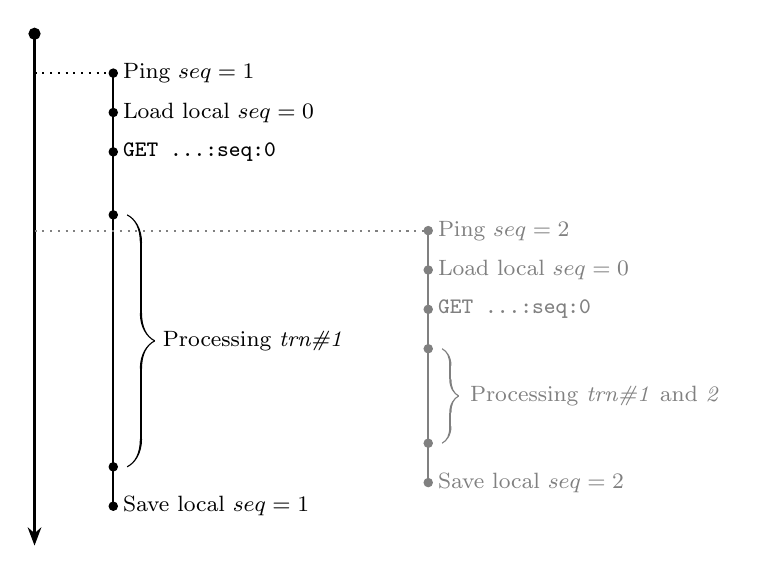
\begin{tikzpicture}
\filldraw[black] (0,0) circle (2pt);
\draw [-Stealth, thick] (0,0) -- (0,-6.5);
\draw [thick, dotted] (0,-0.5) -- (1,-0.5);
\draw [thick] (1,-0.5) -- (1,-6.0);
\filldraw[black] (1,-0.5) circle (1.5pt) node[anchor=west]{\footnotesize Ping $seq=1$};
\filldraw[black] (1,-1.0) circle (1.5pt) node[anchor=west]{\footnotesize Load local $seq=0$};
\filldraw[black] (1,-1.5) circle (1.5pt) node[anchor=west]{\footnotesize \texttt{GET ...:seq:0}};
\filldraw[black] (1,-2.3) circle (1.5pt) node[anchor=west]{};
\draw [decorate, thick, decoration = {calligraphic brace,raise=5pt,amplitude=10pt}] (1,-2.3) -- node[anchor=west]{\hskip0.5cm\footnotesize Processing \textit{trn\#1}} (1,-5.5);
\filldraw[black] (1,-5.5) circle (1.5pt) node[anchor=west]{};
\filldraw[black] (1,-6.0) circle (1.5pt) node[anchor=west]{\footnotesize Save local $seq=1$};
\draw [thick, draw=gray, dotted] (0,-2.5) -- (5,-2.5);
\draw [thick, draw=gray] (5,-2.5) -- (5,-5.7);
\filldraw[gray] (5,-2.5) circle (1.5pt) node[anchor=west]{\footnotesize Ping $seq=2$};
\filldraw[gray] (5,-3.0) circle (1.5pt) node[anchor=west]{\footnotesize Load local $seq=0$};
\filldraw[gray] (5,-3.5) circle (1.5pt) node[anchor=west]{\footnotesize \texttt{GET ...:seq:0}};
\filldraw[gray] (5,-4.0) circle (1.5pt) node[anchor=west]{};
\draw [decorate, thick, pen colour=gray, gray, decoration = {calligraphic brace,raise=5pt,amplitude=6pt}] (5,-4) -- node[anchor=west]{\hskip0.4cm\footnotesize Processing \textit{trn\#1} and \textit{2}} (5,-5.2);
\filldraw[gray] (5,-5.2) circle (1.5pt) node[anchor=west]{};
\filldraw[gray] (5,-5.7) circle (1.5pt) node[anchor=west]{\footnotesize Save local $seq=2$};
\end{tikzpicture}
\end{document}
